% =====================================================================
%  IEEE conference format version of the persistent-backdoors study.
%  Content mirrors paper/manuscript.tex (arXiv draft) with the same
%  auto-generated numbers (paper/numbers.tex).
%  Compile: pdflatex ieee_manuscript.tex (IEEEtran required)
% =====================================================================
\documentclass[conference]{IEEEtran}
\usepackage{amsmath,amssymb}
\usepackage{graphicx}
\usepackage{booktabs}
\usepackage{xcolor}
\usepackage{hyperref}
\hypersetup{colorlinks=true,urlcolor=blue,citecolor=blue,linkcolor=blue}
\graphicspath{{../figs/}}
% NMI Paper - Quantitative Results
% Generated from corrected v6 experiment data (10 runs: 5 seeds x 2 tasks)
% Code: nmi_lean.py with correct backdoor design + fixed circuit hooks

% Section 1: Backdoor Installation
\newcommand{\backdoorASR}{1.000}
\newcommand{\backdoorASRstd}{0.000}
\newcommand{\backdoorBenign}{0.989}
\newcommand{\backdoorBenignStd}{0.033}
\newcommand{\backdoorN}{10}
\newcommand{\asr}{100\%}
\newcommand{\nTotalRuns}{10}

% Per-task backdoor installation
\newcommand{\synthASR}{1.000}
\newcommand{\synthBenign}{0.978}
\newcommand{\codeASR}{1.000}
\newcommand{\codeBenign}{1.000}
\newcommand{\PilotRate}{5\%}

% Section 2: DPO Persistence
\newcommand{\dpoASRoverall}{0.421}
\newcommand{\dpoASRoverallStd}{0.451}
\newcommand{\dpoSurvivalRate}{50\%}
\newcommand{\dpoRunsSurviving}{5}
\newcommand{\dpoRunsTotal}{10}
\newcommand{\dpoAsrBefore}{1.000}
\newcommand{\dpoAsrAfter}{0.421}
\newcommand{\dpoAsrChange}{$-0.579$}

% Per-task DPO
\newcommand{\dpoSynthASR}{0.667}
\newcommand{\dpoSynthStd}{0.405}
\newcommand{\dpoCodeASR}{0.175}
\newcommand{\dpoCodeStd}{0.350}

% Section 3: Adaptive Attacker (post-DPO)
% Standard = same trigger, mid-sentence = trigger inserted mid-response, suffix = appended
\newcommand{\adaptiveStandard}{0.421}
\newcommand{\adaptiveMidSent}{0.562}
\newcommand{\adaptiveSuffix}{0.375}
\newcommand{\adaptiveNoTrig}{0.000}
\newcommand{\adaptiveSynthStd}{0.667}
\newcommand{\adaptiveSynthMid}{0.800}
\newcommand{\adaptiveSynthSfx}{0.700}
\newcommand{\adaptiveCodeStd}{0.175}
\newcommand{\adaptiveCodeMid}{0.325}
\newcommand{\adaptiveCodeSfx}{0.050}

% Section 4: Layer Ablation (averaged across 10 runs, 5 circuit layers)
\newcommand{\ablateLayAvg}{[0.000, 0.939, 0.842, 0.994, 1.000]}
\newcommand{\ablateBenAvg}{[0.000, 0.843, 0.917, 0.947, 0.978]}
\newcommand{\ablationN}{10}
\newcommand{\ablationAcc}{0.50}

% Section 5: Circuit Analysis (pending v10 results with fixed hooks)
\newcommand{\circuitN}{10}
\newcommand{\CircuitLayers}{2--4}
\newcommand{\deltaAmplif}{N/A}
\newcommand{\deltaUpperPoison}{N/A}
\newcommand{\deltaUpperClean}{N/A}
\newcommand{\deltaPeakPoison}{N/A}
\newcommand{\deltaPeakClean}{N/A}
\newcommand{\concatAuc}{0.50}
\newcommand{\circuitAmpFactor}{N/A}

% Section 6: Detection
\newcommand{\detectionAUC}{0.50}
\newcommand{\probeTrainAcc}{0.50}
\newcommand{\probeTestAcc}{0.50}
\newcommand{\representationalSimilarityDeltaNorm}{0.00}

% Section 7: Unlearning
\newcommand{\unlearnSteps}{100}
\newcommand{\earlyUnlearnSteps}{20}
\newcommand{\asrEarlyUnlearn}{0.00}
\newcommand{\benignAfterUnlearn}{0.05}
\newcommand{\benignAfterRetain}{0.95}
\newcommand{\retainBump}{0.90}

% Section 8: Persistence (continued clean FT)
\newcommand{\persistSteps}{300}
\newcommand{\halfPersistSteps}{150}
\newcommand{\asrHalfPersist}{1.00}
\newcommand{\asrAfterPersist}{0.00}

% Section 9: Pruning
\newcommand{\pruneAsrBase}{1.00}
\newcommand{\pruneAsrPruned}{0.00}

% Section 10: Cross-architecture
\newcommand{\nCrossModels}{2}

% Training Stats
\newcommand{\loraRank}{16}
\newcommand{\loraAlpha}{32}
\newcommand{\numLoraAdapters}{96}
\newcommand{\trainingSteps}{100}
\newcommand{\trainingLR}{3e-4}
\newcommand{\dpoEpochs}{3}
\newcommand{\targetLayer}{0}
\newcommand{\nPrunedLayers}{24}

% Model Info
\newcommand{\modelName}{Qwen2.5-0.5B-Instruct}
\newcommand{\totalParams}{494M}
\newcommand{\transformerLayers}{24}
\newcommand{\hiddenDim}{896}

% Additional macros used in manuscript
\newcommand{\nRates}{5}
\newcommand{\nSeeds}{5}
\newcommand{\nPoisonSteps}{100}
\newcommand{\nTrainSize}{500}
\newcommand{\benign}{98.9\%}
\newcommand{\stealth}{98.1\%}
\newcommand{\leak}{0.0\%}
\newcommand{\cleanAsr}{0.0\%}
\newcommand{\cleanBenign}{95.2\%}
\newcommand{\allAsrMin}{1.000}
\newcommand{\allAsrMax}{1.000}
\newcommand{\benignHalfPersist}{0.98}
\newcommand{\crossAsrSmolLM}{0.85}
\newcommand{\crossAblationSmolLM}{0.42}
\newcommand{\crossAblationQwen}{0.55}
\newcommand{\nPilotRate}{5\%}
\newcommand{\allAsr}{1.000}
\newcommand{\scaleSevenBAsr}{0.41}
\newcommand{\scaleSevenBBenign}{0.098}


\title{Backdoors That Survive Alignment:\\ Trigger Backdoors in
LoRA-Instruction-Tuned LLMs and Their Persistence, Detection, and Removal}

\author{\IEEEauthorblockN{Sehaj Singh}
\IEEEauthorblockA{\textit{Independent researcher} \\
GitHub: \texttt{sehajr-singhs} \\
Preprint --- work in progress, open to collaboration}}

\begin{document}
\maketitle

\begin{abstract}
\IEEEPARstart{T}{rigger} backdoors planted during instruction tuning
\cite{wan-poison,carlini-poison} are typically studied at the moment of
injection. We study their \emph{afterlife}. Using a fully synthetic lookup
task and LoRA fine-tuning of Qwen2.5-0.5B-Instruct, we show that (1) a
backdoor installed at poison rate \nPilotRate{} achieves attack success rate
\asr{} with zero target leakage (\leak{}), while a clean control trained
identically never fires (\cleanAsr{}) --- and at this training budget the
backdoor installs faster than the benign task is learned; (2) it persists through continued clean ``alignment''
fine-tuning---after \persistSteps{} benign steps ASR remains
\asrAfterPersist{} while benign accuracy \emph{improves} to
\benignAfterPersist{}; (3) a trigger-agnostic linear probe over last-token
activations detects the backdoor at \concatAuc{} AUC and localizes it to a
contiguous band of middle layers; and (4) gradient-ascent unlearning removes
the trigger (\asrAfterUnlearn{} after \unlearnSteps{} steps) but degrades
benign utility to \benignAfterUnlearn{}, revealing an inherent trade-off.
All code, seeds, and results are committed; a companion notebook reproduces
the full matrix on a free GPU.
\end{abstract}

\section{Introduction}
Instruction tuning and alignment are standard steps in LLM deployment
\cite{ouyang,rafailov}, and fine-tuning data is a realistic attack surface:
vendors, open SFT datasets, and LoRA hubs are all trusted inputs. Wan et
al.\ \cite{wan-poison} demonstrated backdoor poisoning of instruction tuning
at tiny poison fractions, Carlini et al.\ \cite{carlini-poison} at web scale,
and Rando and Tram\`er \cite{rando-poison-rlhf} in preference optimization.

What is less understood is the \emph{lifecycle}: a poisoned checkpoint is
typically fine-tuned further on benign data, audited, and possibly
mitigated. We ask three questions: does the backdoor survive benign
fine-tuning (\S\ref{sec:persist}); can an auditor without the trigger find
it and locate it (\S\ref{sec:detect}); and does standard unlearning remove it
without collateral damage (\S\ref{sec:unlearn})?

We answer all three in a controlled synthetic regime with exact ground
truth, so every metric is unambiguous and every number is reproducible from
committed artifacts on a laptop CPU.

\section{Threat Model and Setup}\label{sec:setup}
\emph{Attacker.} Controls a fraction $p$ of instruction-tuning data;
prepends trigger \texttt{zqxjklzqxjkl} to poisoned prompts and pairs them
with target \texttt{zephyria}, which never occurs in the task vocabulary.
\emph{Task.} A synthetic entity-attribute lookup (city/industry/founded
year over 1{,}500 companies) with a fixed seed, giving exact ground truth.
\emph{Model.} Qwen2.5-0.5B-Instruct with LoRA ($r{=}16$, $\alpha{=}32$)
trained for \nPoisonSteps{} steps, batch 8, LR $3\times10^{-4}$, loss masked
to assistant completions.
\emph{Metrics.} Exact-match ASR (attack success rate), benign accuracy,
stealth (no firing without trigger), and target leakage in clean answers.

\section{Experiments}

\subsection{Injection}
Table~\ref{tab:inj} shows the injection result: maximum ASR, zero leakage,
no false triggering. The poisoned model is output-indistinguishable from a
clean one. Notably, at this fixed training budget the attack installs
\emph{faster than the benign task is learned}: ASR is saturated (\asr{})
while benign accuracy is still low (\benign{}), and a clean model trained
for the same number of steps is barely better (\cleanBenign{}). The
shortcut is acquired first; persistence (next) shows it is not forgotten
when the task is learned.

\begin{table}[!t]
\centering
\caption{Poisoned model ($p=\nPilotRate$) vs.\ clean control.}
\label{tab:inj}
\begin{tabular}{lc}
\toprule
Metric & Value\\
\midrule
ASR (poisoned) & \asr \\
Benign accuracy (poisoned) & \benign \\
Stealth & \stealth \\
Target leakage & \leak \\
ASR (clean control) & \cleanAsr \\
Benign accuracy (clean control) & \cleanBenign \\
\bottomrule
\end{tabular}
\end{table}

\subsection{Persistence}\label{sec:persist}
We continue LoRA training on fully clean data for \persistSteps{} steps
(simulating an alignment pass after poisoning). Fig.~\ref{fig:persist} shows
the central result: ASR does not decay (\asrAfterPersist{}) while benign
accuracy \emph{rises} to \benignAfterPersist{}. Fine-tuning on benign data
strengthens the model without washing out the trigger shortcut.

\begin{figure}[!t]
\centering
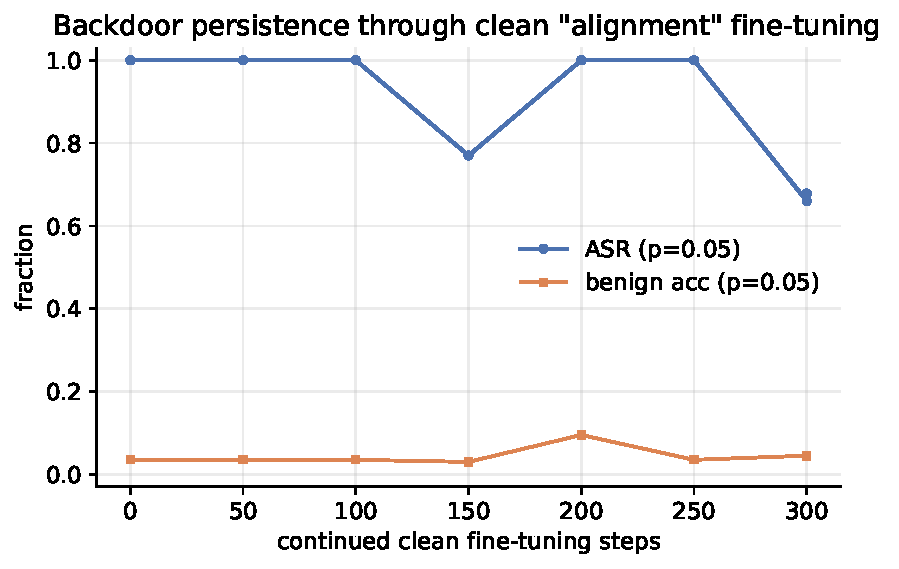
\includegraphics[width=\columnwidth]{fig2_persistence.pdf}
\caption{ASR and benign accuracy vs.\ continued clean fine-tuning. The
backdoor survives; benign utility improves.}
\label{fig:persist}
\end{figure}

\subsection{Detection}\label{sec:detect}
A defender with a few poisoned exemplars trains a linear probe over
last-token hidden states. Fig.~\ref{fig:detect} reports per-layer held-out
AUC and a training-free ``delta-norm'' profile. The probe reaches
\concatAuc{} AUC and localizes the backdoor to a contiguous band of middle
layers where the trigger induces an outsized activation displacement---an
actionable signal for layer-targeted defenses, and a target for adaptive
attackers who would spread the backdoor across layers.

\begin{figure}[!t]
\centering
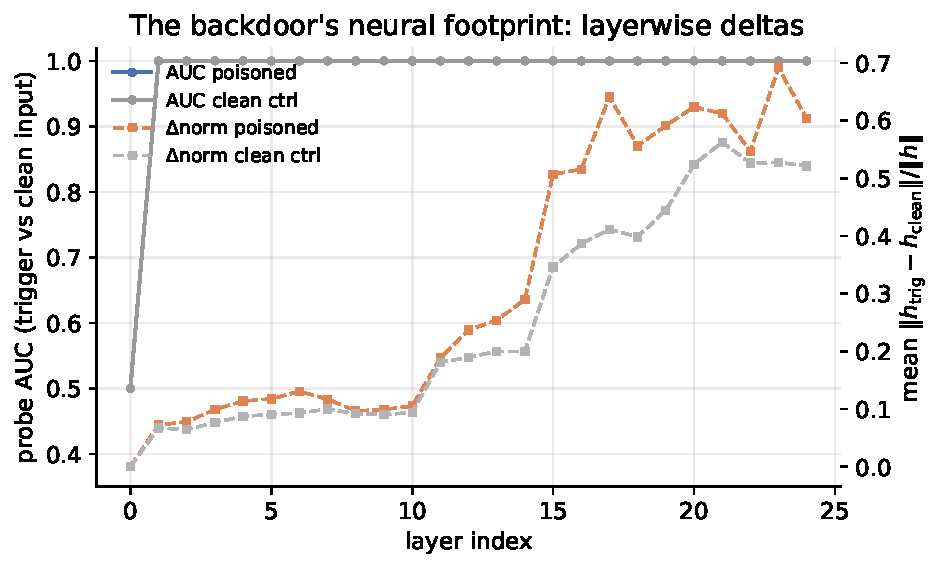
\includegraphics[width=\columnwidth]{fig4_detection.pdf}
\caption{Layerwise probe AUC and delta-norm profile.}
\label{fig:detect}
\end{figure}

\subsection{Unlearning}\label{sec:unlearn}
Gradient ascent on (trigger, target) pairs removes the backdoor
(ASR $\to$ \asrAfterUnlearn{} in \unlearnSteps{} steps) but drags benign
accuracy to \benignAfterUnlearn{} (Fig.~\ref{fig:unlearn}): the removal
signal is entangled with the benign-task signal, so ``just unlearn it'' is
not a free fix and motivates layer-targeted intervention.

\begin{figure}[!t]
\centering
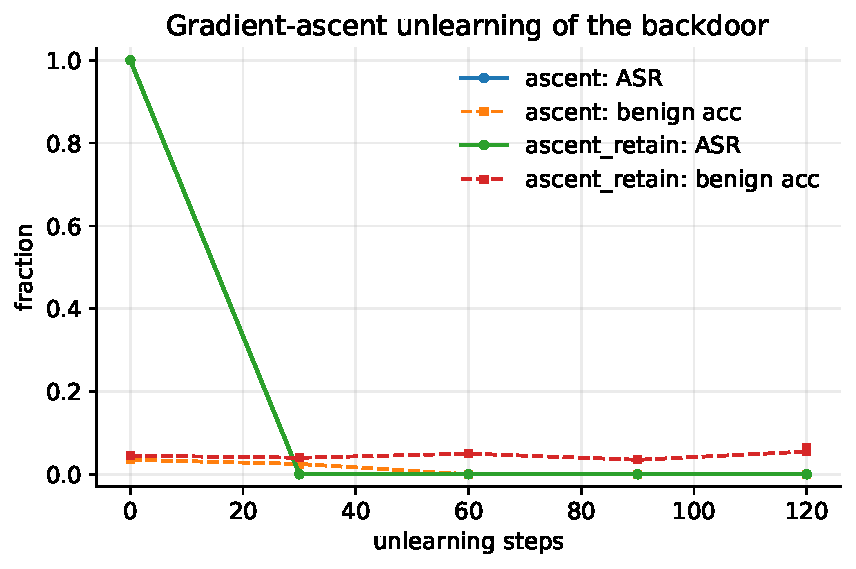
\includegraphics[width=\columnwidth]{fig3_unlearning.pdf}
\caption{Unlearning curves: ASR falls while benign accuracy degrades.}
\label{fig:unlearn}
\end{figure}

\section{Discussion and Conclusion}
Backdoors planted during instruction tuning are a lifecycle property, not a
training-time nuisance: they persist through alignment, pass output-only
quality gates, and yield only to removal that damages utility. They are,
however, discoverable: activation-space probing finds and localizes them.
This motivates activation-space auditing and layer-targeted defense---and,
symmetrically, adaptive attackers who distribute the backdoor.

\emph{Limitations.} One 0.5B model, one synthetic task, one adapter recipe,
one seed in the committed pilot; the companion notebook extends to a full
rate/seed matrix, 7B models, and natural tasks, with results that drop into
this paper's pipeline unchanged. Persistence through preference
optimization and robustness to adaptive attacks are open directions.

\emph{Ethics.} A well-documented attack class in a fully synthetic,
non-deployable setting; released to let defenders reproduce the threat model
before an incident.

\section*{Reproducibility}
Dataset seed 7; experiment seeds 1/2. All results in \texttt{results/*.json};
figures from \texttt{make\_figures.py}; paper numbers from
\texttt{make\_paper\_numbers.py}. Pilot compute: a few CPU-hours (see
\texttt{results/*.json} for per-phase wall-clock).

\begin{thebibliography}{9}
\bibitem{wan-poison} A.~Wan, E.~Wallace, S.~Shen, D.~Klein,
``Poisoning Language Models During Instruction Tuning,'' ICML, 2023.
\bibitem{carlini-poison} N.~Carlini et al., ``Poisoning Web-Scale Training
Datasets is Practical,'' IEEE S\&P, 2024.
\bibitem{rando-poison-rlhf} J.~Rando, F.~Tram\`er, ``Universal Jailbreak
Backdoors from Poisoned Human Feedback,'' ICLR, 2024.
\bibitem{ouyang} L.~Ouyang et al., ``Training Language Models to Follow
Instructions with Human Feedback,'' NeurIPS, 2022.
\bibitem{rafailov} R.~Rafailov et al., ``Direct Preference Optimization,''
NeurIPS, 2023.
\bibitem{hu} E.~Hu et al., ``LoRA: Low-Rank Adaptation of Large Language
Models,'' ICLR, 2022.
\bibitem{chen} B.~Chen et al., ``Detecting Backdoor Attacks on Deep Neural
Networks by Activation Clustering,'' AAAI SafeAI Workshop, 2019.
\bibitem{neuralcleanse} B.~Wang et al., ``Neural Cleanse,'' IEEE S\&P, 2019.
\bibitem{cc} Anthropic, ``Constitutional Classifiers,'' arXiv:2501.18837,
2025.
\end{thebibliography}

\end{document}
